\section{人間の諸特性}
本章では2、、、

\subsection{身体的特性}
本節では2、、、

\subsubsection{静的形態特性}
本項では2、、、

\begin{table}[h]
\centering
\caption{PTS法(MODAPT法)による動作時間の例}
\label{MODAPT}
\begin{tabular}{cccc}
\toprule
移動時間 [cm] & 身体部位 & 動作時間 [sec] & 比率 \\
\midrule
約2.5 & 指 & 0.129 & 1 \\
約5 & 手首から先 & 0.258 & 2 \\
約15 & 前腕 & 0.387 & 3 \\
\bottomrule
\end{tabular}
\end{table}

箇条書きの例。
\begin{itemize}
\item ユーザの許容範囲の共通範囲を採用する(例:自動販売機)
\item 立場の弱いユーザに合わせる(例:公園の水飲み場)
\end{itemize}

立場の弱いユーザに合わせる場合や,ユーザ層ごとに設計する場合には,
全体として5\textasciitilde95\%ileのユーザを保証しなければならない.
なお,\emph{安全性に関わる部分では1\textasciitilde99\%ileのユーザを保証する必要がある.}

\begin{figure}[h]
\centering
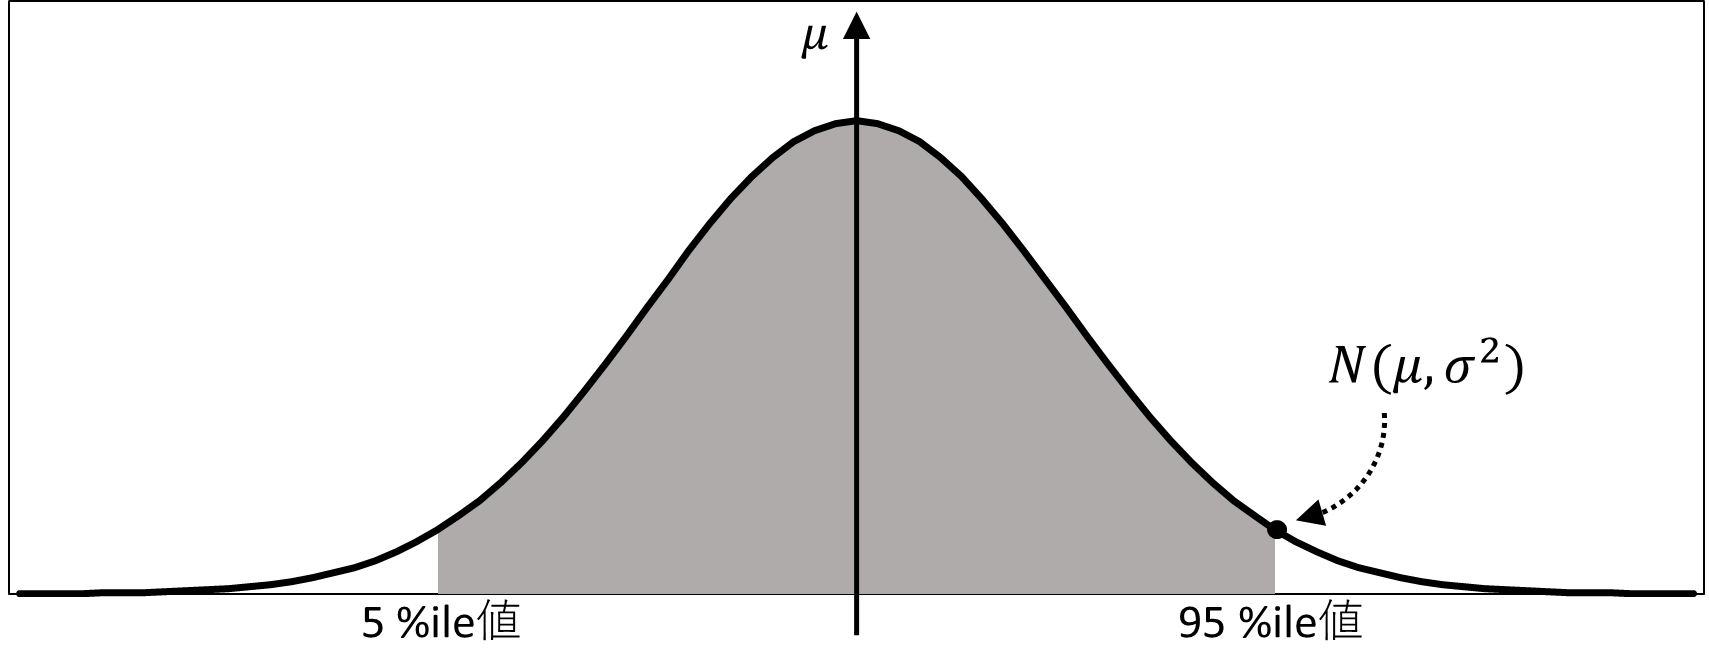
\includegraphics[width=13cm]{img/fig.png}
\caption{パーセンタイル}
\end{figure}

